\documentclass{article}

\usepackage{graphicx}
\usepackage{tikz}
\usepackage{tikzsymbols}
\usetikzlibrary{calc,patterns,shapes.geometric}
\pagestyle{empty}
\usepackage[margin=0pt]{geometry}
\geometry{papersize={14in,12in}}

\def\centerarc[#1](#2)(#3:#4:#5){\draw[#1] ($(#2)+({#5*cos(#3)},{#5*sin(#3)})$) arc (#3:#4:#5);}

\begin{document}
	\begin{figure}
		\centering
		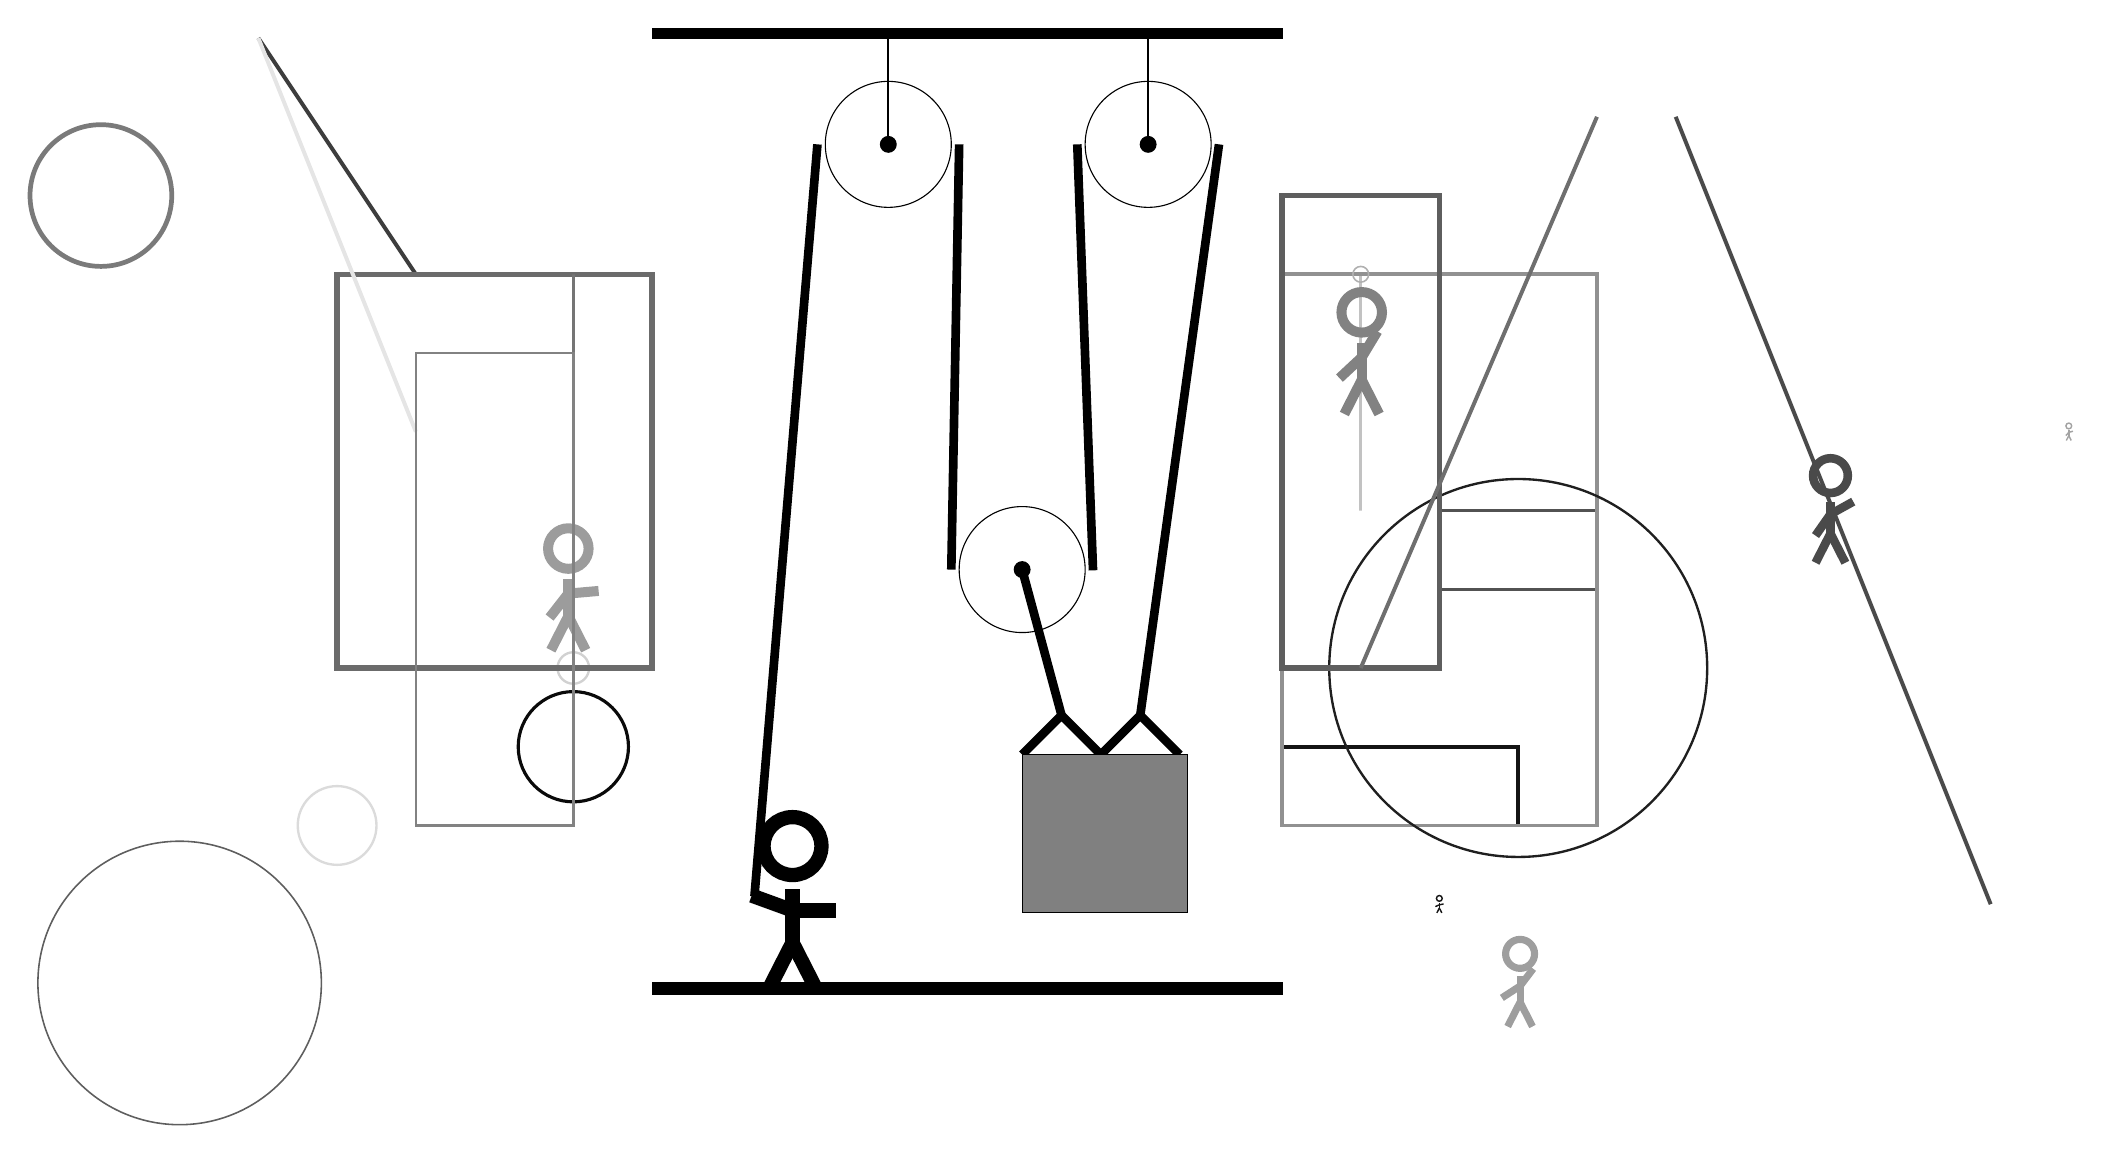
\begin{tikzpicture}
			%%%%% START %%%%%
			
			\draw[fill=black] (-2, 9) rectangle (6, 9.125);
			
			\draw (1, 7.65) circle (0.8);
			\draw[fill=black] (1, 7.65) circle (0.1);
			\draw[thick] (1, 7.65) -- (1, 9);
			
			\draw (4.3, 7.65) circle (0.8);
			\draw[fill=black] (4.3, 7.65) circle (0.1);
			\draw[thick] (4.3, 7.65) -- (4.3, 9);
			
			\draw (2.7, 2.25) circle (0.8);
			\draw[fill=black] (2.7, 2.25) circle (0.1);
			
			\draw[line width=1.1mm]  (2.7, -0.1) -- (3.2, 0.4) -- (3.7, -0.1) -- (4.2, 0.4) -- (4.7, -0.1);
			\draw[fill=black!50] (2.7, -0.1) rectangle (4.8, -2.1);
			
			\draw[line width=0.4mm, color=black!24] (7, 3) rectangle (7, 6);
			
			\draw[line width=0.5mm, color=black!92] (6, 0) rectangle (9, -1);
			\draw[line width=0.4mm, color=black!68] (8, 3) rectangle (10, 2);
			\draw[line width=0.5mm, color=black!43] (6, 6) rectangle (10, -1);
			\node[line width=0.4mm, color=black!38] at (9, -3) {\Strichmaxerl[5][33][53]};
			\draw[line width=0.5mm, color=black!76](-7, 9) -- (-5, 6);
			\draw [line width=0.4mm, color=black!96](-3, 0) circle (0.7);
			
			\draw [line width=0.3mm, color=black!18](-3, 1) circle (0.2);
			\node[line width=0.5mm, color=black!71] at (13, 3) {\Strichmaxerl[6][55][29]};
			\draw [line width=0.3mm, color=black!88](9, 1) circle (2.4);
			\draw[line width=0.7mm, color=black!63] (8, 1) rectangle (6, 7);
			\draw [line width=0.2mm, color=black!31](7, 6) circle (0.1);
			\draw [line width=0.3mm, color=black!14](-6, -1) circle (0.5);
			\draw[line width=0.7mm, color=black!58] (-2, 6) rectangle (-6, 1);
			\draw[line width=0.5mm, color=black!71](11, 8) -- (15, -2);
			\draw[line width=0.5mm, color=black!10](-7, 9) -- (-5, 4);
			\node[line width=0.2mm, color=black!91] at (8, -2) {\Strichmaxerl[1][24][11]};
			\draw[line width=0.5mm, color=black!68](8, 8) -- (8, 8);
			\draw [line width=0.6mm, color=black!52](-9, 7) circle (0.9);
			
			\node[line width=0.5mm, color=black!36] at (16, 4) {\Strichmaxerl[1][47][16]};
			\node[line width=0.2mm, color=black!39] at (-3, 2) {\Strichmaxerl[7][52][5]};
			
			\draw[line width=0.3mm, color=black!54] (-3, 1) rectangle (-3, 6);
			
			\draw[line width=0.3mm, color=black!49] (-3, -1) rectangle (-5, 5);
			\node[line width=0.4mm, color=black!49] at (7, 5) {\Strichmaxerl[7][43][59]};
			\draw [line width=0.2mm, color=black!63](-8, -3) circle (1.8);
			\draw[line width=0.5mm, color=black!57](7, 1) -- (10, 8);
			
			
			\draw[line width=1.1mm](-0.7, -1.9) -- (0.1, 7.65);
			\centerarc[line width=1.1mm](1, 7.65)(0:180:0.9);
			\draw[line width=1.1mm](1.9, 7.65) -- (1.8, 2.25);
			\centerarc[line width=1.1mm](2.7, 2.25)(180:370:0.9);
			\draw[line width=1.1mm] (3.6, 2.24) -- (3.4, 7.65);
			\centerarc[line width=1.1mm](4.3, 7.65)(0:180:0.9);
			\draw[line width=1.1mm](4.2, 0.4) -- (5.2, 7.65);
			\draw[line width=1.1mm] (3.2, 0.4) -- (2.7, 2.25);
			
			\node at (-0.2, -2) {\Strichmaxerl[10][-20][0]};
			
			\draw[fill=black] (-2, -3) rectangle (6, -3.15);
			
			%%%%% END %%%%%
		\end{tikzpicture}
	\end{figure}	
\end{document}